\documentclass[conference]{IEEEtran}
% \IEEEoverridecommandlockouts
% The preceding line is only needed to identify funding in the first footnote. If that is unneeded, please comment it out.
\usepackage{cite}
\usepackage{amsmath,amssymb,amsfonts}
% \usepackage{algorithmic}
\usepackage{graphicx}
\usepackage{textcomp}
\usepackage{xcolor}
\usepackage{algorithm}
\usepackage{booktabs}       % professional-quality tables
\usepackage{algorithm}
\usepackage{algpseudocode}
\usepackage{hyperref}
\usepackage{layout}
\usepackage{listings}
\usepackage[utf8]{inputenc}

\graphicspath{{"../results/"}}
\def\BibTeX{{\rm B\kern-.05em{\sc i\kern-.025em b}\kern-.08em
    T\kern-.1667em\lower.7ex\hbox{E}\kern-.125emX}}
\begin{document}

\title{battery-charger: Reinforcement learning techniques for wholesale market participation of grid-scale batteries}

\author{\IEEEauthorblockN{Erich Trieschman}
\IEEEauthorblockA{\textit{Department of Statistics} \\
\textit{Stanford University}\\
Stanford, CA \\
etriesch@stanford.edu}
}

\lstset{frame=tb, language=Python,
  aboveskip=3mm,
  belowskip=3mm,
  showstringspaces=false,
  columns=flexible,
  basicstyle={\small\ttfamily},
  numbers=none,
  numberstyle=\tiny\color{gray},
  keywordstyle=\color{blue},
  commentstyle=\color{dkgreen},
  stringstyle=\color{mauve},
  breaklines=true,
  breakatwhitespace=true,
  tabsize=3}

\maketitle

\begin{abstract}
    This paper analyzes the revenue potential of long and short-term batteries. First, I compare the theoretical bounds (optimal and naive) across battery durations. Next, I compare the performance of various reinforcement learning algorithms across the same durations.
\end{abstract}

\section{Introduction}
Grid-scale batteries will play a critical role in our grid's transition to renewable energy. By capturing surplus renewable energy and dispatching it in shortages, they help reduce a grid's reliance on thermal power and lessen the physical demands on transmission lines. In this way, batteries are both load centers and generators of power and a battery schedule in one time period affects the available options at subsequent time periods \cite{IEA}. 

Prices for electricity at each node in the grid are settled in real time every 15 and 5 minutes \cite{CAISO}. The optimal operating schedule can only be learned in hindsight, yet effective battery charge can still lead to meaningful revenue. The main challenge with battery management is price uncertainty. A battery operator must decide how to charge and discharge his/her battery given the available information so as to maximize the expected cummulative returns. 

A further decision includes which type of battery to use: a long duration battery that can charge and discharge over the course of several days, or a short duration battery that charges and discharges over the course of several hours. While long duration batteries can use strategic reseves to dispatch more at optimal times, they are also less efficient, so gains from improved arbitrage may be offset by roundtrip charging losses.

This paper analyzes the revenue potential of long and short-term batteries. First, I compare the theoretical bounds (optimal and naive) across battery durations. Next, I compare the performance of various reinforcement learning algorithms across the same durations.

\section{Methods: Data and parameters}
\subsection{Data}
My analysis studies battery performance within the California wholesale electricity market. This wholesale market is operated by the California Independent System Operator (CAISO), which clears real-time electricity prices at every node on the grid every 5 and 15 minutes. CAISO data is publicly available and I use the `gridstatus' package to access the 15-minute realtime market and the 1-hour day ahead market data. I consider data at these nodes from 2020 through 2022 \cite{Gridstatus}.

There are over 1594 nodes in the CAISO market with available price data. To capture potential heterogeneity across the state, my analysis extends to four representative nodes. Two actual nodes, one in the northern zone (NP15) and one in the Southern zone (SP15), and two trading hubs. The two actual nodes I select correspond to two of PG\&E's major battery projects within CAISO \cite{Colthorpe} \cite{IEA}, one identified as proximate to a large solar installation, and the other proximate to a large generator with existing transmission. The trading hubs are virtual hubs, developed by CAISO, to represent the average price paid to generation resources within Existing Zones to support hedging \cite{CAISO_trade}. Table \ref{tab:caiso} provides more details on these hubs.

\begin{table}[htbp]
    \caption{\label{tab:caiso} CAISO nodes}
    \begin{center}
        \begin{tabular}{llll}
            \hline
            \textbf{Node} & \textbf{Location} & \textbf{Capacity} \\
            \hline
            SANDLOT\_2\_N022 & Mojave, Kern Cty. & 169MW\/676MWh \\
            MOSSLDB\_2\_B1 & Moss Landing, Monterey Ct. & 350MW\/1400MWh \\
            TH\_NP15\_GEN\-APND & N. Trading Zone & - \\
            TH\_SP15\_GEN\-APND & S. Trading Zone & - \\
            \hline
        \end{tabular}
    \end{center}
\end{table}

I reserve 2022 as my analysis year to evaluate the performance of various charging strategies. I use 2020 and 2021 data for cross validation and hyper-parameter tuning.

\subsection{Battery parameters}
My analysis uses battery parameters described in Table \ref{tab:battery}. I base power capacity on the average of upcoming PG\&E grid-scale battery projects \cite{Colthorpe} \cite{IEA}. Duration and round-trip efficiency parameters were set in conversations with experts in grid-scale battery storage. 
\begin{table}[htbp]
    \caption{\label{tab:battery} Battery parameters}
    \begin{center}
        \begin{tabular}{ll}
            \hline
            \textbf{Parameter} & \textbf{Value}\\
            \hline
            Power capacity (MW) & 200\\
            Duration (hr) & \{4, 24, 100\}\\
            Energy capacity (MWh) & Power capacity * Duration \\
            Efficiency (\%) & 92.5 (12hr); 86 (24hr); 70 (100hr)\\
            \hline
        \end{tabular}
    \end{center}
\end{table}


% -------------------------------------------------
% <><><><><><><>    BASELINES
% -------------------------------------------------
\section{Methods: Baseline performance}
I calculate two baselines to bound the expected performance of my reinforcement learning approaches. As an upper bound, I use linear optimization to calculate the maximum-revenue strategy; as a lower bound, I implement a naive rule of charging during non-peak hours and dispatching during peak hours. 

\subsection{Optimal baseline}
With known prices, energy arbitrage can be framed as a convex optimization problem; this has been well studied  and can be formulated with an objective and constraints as follows \cite{boyd}:

\begin{align*}
    \max_{c, d}\;\; & p^T(\nu d - \frac{1}{\nu}c)\\
    s.t\;\; & E_{[1:T]} = E_{[0:T-1]} + c_{[0:T-1]} - d_{[0:T-1]}\\
    & 0 \preceq E \preceq E_{max}\\
    & C_{min} \preceq c \preceq C_{max}\\
    & D_{min} \preceq d \preceq D_{max}
\end{align*}

Where $c, d \in \mathbb{R}^T$ are charge and discharge quantities in each period, $t$. $p \in \mathbb{R}^T$ is realtime prices in those corresponding periods. $E_{max}, C_{min}, C_{max}, D_{min}, D_{max} \in \mathbb{R}$ are physical constraints on total energy capacity and charge/discharge power capacity respectively. $\nu \in \mathbb{R}$ is the efficiency of charging and discharging. Note that physical constraints and efficiency vary by battery duration.

\subsection{Optimal baseline under 10-day foresight}
As a slightly tighter upper bound, I also calculate the optimal battery performance under 10-day forecast windows. Given best weather and price forecasts extend out only 10 days, this theoretical upper bound may represent performance closer to (but still likely above), the performance of reinforcement learning models.

\subsection{Naive baseline}
Given trends in energy use and reports of the net load curve in California, I develop a naive baseline set through simple charge and discharge rules throughout the day \cite{CAISO}. Figure \ref{fig:mp} shows mean price at every 15 minute interval throughout the day; I use this figure to choose the specific thresholds for my charge and discharge rules, which are the same across battery durations. I provide the naive baseline charging schedule in Table \ref{tab:naive}.

\begin{figure}[htbp]
    \caption{\label{fig:mp} Mean hourly price across nodes, 2020-2022}
\centerline{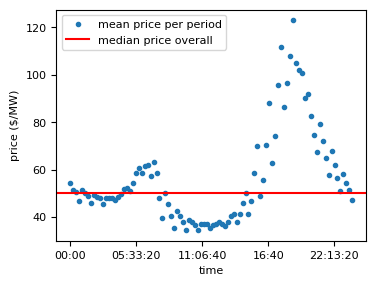
\includegraphics[width=.8\linewidth]{mean_price.png}}
\end{figure}


\begin{table}[htbp]
    \caption{\label{tab:naive} Naive baseline schedule}
    \begin{center}
        \begin{tabular}{clc}
            \hline
            \textbf{Time} & \textbf{Action} & \textbf{Storage} \\
            \hline
            00:00 - 02:00 & - & 0 \\
            02:00 - 04:00 & Charge & 2 * Capacity \\
            04:00 - 08:00 & - & 2 * Capacity \\
            08:00 - 10:00 & Discharge & 0 \\
            10:00 - 11:00 & - & 0 \\
            11:00 - 15:00 & Charge & 4 * Capacity \\
            15:00 - 17:00 & - & 4 * Capacity \\
            17:00 - 21:00 & Discharge & 0 \\
            21:00 - 00:00 & - & 0 \\
            \hline
        \end{tabular}
    \end{center}
\end{table}

\section{Methods: Reinforcement learning}
I use reinforcement learning algorithms from AA228: Decision Making under Uncertainty to develop revenue-maximizing battery schedules \cite{kochenderfer}. I implement a model-based and a model-free Markov decision process problem (MDPs). In the sections below, I describe the structure of these problems, as well as my approach for model selection and hyperparameter tuning.

\subsection{Action space and reward function}
Consistent across both MDPs are my action space and reward function. The actions I consider are Charge, Discharge, and No Action. In any period, $t$, I take only one action $\in (c_t, d_t, 0)$, where
\begin{align*}
    \textrm{Charge: } c_t &= \min(C_{max}, E_{max} - E_{t-1})\\
    &= \min(200MW, 200MW*Duration - E_{t-1})\\
    \textrm{Discharge: } d_t &= \min(D_{max}, E_{t-1} - E_{min})\\
    &= \min(200MW, E_{t-1})\\
    \textrm{No action: } &= 0
\end{align*}

I find that a reward function based solely on revenue in each time period is not sufficient to incentivize exploration of my state space. Intuitively, this is because greedy actions always prefer revenue-generating discharge or revenue-maintaining no-action over revenue-losing charge. Wang et al. also finds that this method leads to under-exploring of the state-space and makes significant by incorporating a moving average into the reward function \cite{Wang}. From the optimal baseline analysis, I also observe that longer-duration batteries' optimal performance involves maintaining partial storage throughout the period. My final reward function includes elements of these three benefits. 

The revenue component follows the optimization problem above:
\begin{align}
    REV(s, a) = p_t * \left(\nu * d_t - \frac{1}{\nu}*c_t\right)
\end{align}

The moving average component rewards charging and penalizes discharging when the current price drops below the moving average; when current price rises above the moving average, the incentives are reversed:

\begin{align}
    MA(s, a) = \begin{cases}
        (pma_t - p_t) * 200 & \textrm{if charge}\\
        (p_t - pma_t) * 200 & \textrm{if discharge}\\
        0 & \textrm{else}
    \end{cases}
\end{align}

Lastly, the energy component rewards next-period's storage:

\begin{align}
    ES(s, a) = \begin{cases}
        e_t + 200 & \textrm{if charge}\\
        e_t - 200 & \textrm{if discharge}\\
        e_t & \textrm{else}
    \end{cases}
\end{align}

My reward function is a weighted average of these three components:
\begin{align*}
    R(s_t, a) &= \phi_r REV(s_t, a) + \phi_m MA(s_t, a) + \phi_e ES(s_t, a)\\
    \textrm{where } & 0 \preceq \phi \preceq 1\\
    & \phi^T 1 = 1
\end{align*}

I treat $\phi$, the weighting of these three rewards, as a hyperparameter which I tune through crossvalidation.

\subsection{Model-free approach}
For a model-free approach, I use Q-learning with $\epsilon$-greedy exploration and a discretized state space. This approach is an offline, model-free approach because I learn the value function offline prior to deploying my strategy, and I make no assumptions about the transition function. I use observations from historical data (from 2020 and 2021) to iteratively learn the value function and an optimal policy. Q-learning is a standard explore-exploit approach where I balance exploring unseen states (i.e., different charges under different price conditions) with exploiting greedy behavior (i.e., discharging to make revenue).

Q-learning requires a discrete state-space. My state space consists of the following discrete quantities
\begin{itemize}
    \item $S_{rt}$: Real-time prices, discretized by quantile into 100 bins
    \item $S_{m}$: Month of year
    \item $S_{w}$: Weekday indicator
    \item $S_{h}$: Hour of day
    \item $S_{e}$: State of charge of battery, discretized into 50MW units
\end{itemize}

The Q-learning algorithm iterates until convergence. In each iteration, I perform batch updates of the Q-function (the value function under every action) using batches of samples, instead of a single sample point at a time. And within each batch, I iterate over every possible energy state of the battery, to improve the estimate of the value at every state of charge of the battery. I find that the Q-function converges in roughly 25 iterations and I use a batch size of 300 sample points.

In this algorithm, I define a few hyperparameters, which I tune through cross validation. Those hyperparameters are
\begin{itemize}
    \item $\alpha$: the learning rate
    \item $\epsilon$: the probability of exploring (instead of taking the optimal action under the current Q-function)
    \item $\psi$: a control on the decay of $\epsilon$ over time, $t$, where I decay $\epsilon$ by $\exp(-t * \psi)$
\end{itemize}

\subsection{Model-based approach}
For a model-based approach, I approximate a transition function, $T(s_{t+1} \mid s_t, a)$, using a time-series model and a value function, $U^\pi(s) = \theta^TB(s)$ through linear regression. With this approach I can work with a continuous state space. My state space consists of the following quantities
\begin{itemize}
    \item $PRT$: Real-time prices
    \item $PDA$: Day-ahead prices (reported for every hour of the day)
    \item $M$: Month of year
    \item $W$: Weekday indicator
    \item $H$: Hour of day
    \item $E$: State of charge of battery, discretized into 50MW units
\end{itemize}

 Note $PDA$ is deterministic because day ahead prices are settled the day prior to trading; hence, next hour's price is known at the beginning of the day. $M,W,H$ have known, deterministic, transitions, as does $E$, which evolves depending on the decision to charge, discharge, or do nothing. Therefore, under this state space the only uncertain transition state is that of $PRT$, which I use time-series modeling to estimate; I include lag and square terms to better approximate the series. I present the results of this model in Tables \ref{tab:ts1} and \ref{tab:ts2} and Figure \ref{fig:ts} in the Appendix (Section \ref{sec:taf}).

 In my model-based approximation of the value function, I approximate a unique value function for every energy state. Hence
 \begin{align*}
    U(s_t) &= U(PRT_t, PDA_t, M_t, W_t, H_t, E_t)\\
    &= U_{e = E_t}(PRT_t, PDA_t, M_t, W_t, H_t)\\
    &= \theta_{e = E_t}^T B(PRT_t, PDA_t, M_t, W_t, H_t)
 \end{align*}

 And under the transition states above, assuming a normally distributed error for my time-series model, I have
 \begin{align*}
    E[U(s_{t+1})] &= \theta_{e = E_t+1}^T B(E[PRT_{t+1}], PDA_{t+1}, M_{t+1}, W_{t+1}, H_{t+1})\\
    &= \theta_{e = E_t+1}^T B(\hat{PRT_{t+1}}, PDA_{t+1}, M_{t+1}, W_{t+1}, H_{t+1})\\
    &= \theta_{e = E_t+1}^T B(\hat{s}_{[-E]t+1})
 \end{align*}

 This leads to the following value iteration
 \begin{align*}
    U^{(i+1)}(s_t) &\leftarrow R(s,a) + \gamma * E_{T(s_{t+1}\mid s, a)}[U^{(i)}(s_{t+1})]\\
    &\leftarrow R(s,a) + \gamma * \theta_{e = E_t+1}^T B(\hat{s}_{[-E]t+1})
 \end{align*}


\section{Results \label{sec:results}}
In this section I present my results. Table \ref{tab:summary} presents the overall performance of baseline and reinforcement learning schedules, across the 4 nodes and 3 durations that I consider. Figure \ref{fig:summ4} displays the performance of each schedule over time for the 4-hour duration battery at the Moss Landing node and Figure \ref{fig:summ100} displays the same for the 100-hour duration battery.

I am still tuning the hyperparameters for my reinforcement learning algorithms. The results in this section reflect initial guesses for all hyperparameters.

\begin{table}[htbp]
    \caption{\label{tab:summary} Overall performance by schedule, duration, and node}
    \begin{center}
        \begin{tabular}{lrrrrrc}
            \toprule
             \textbf{Node} & \textbf{Dur.} &  \textbf{naive} &  \textbf{10d opt.} &  \textbf{optimal} &  \textbf{Q-learn} & \textbf{V-it.} \\
            \midrule
            TH\_NP15         & 4hr &   12.1 &              25.8 &     25.7 &  -30.3 &     - \\
            (GEN-APND)       & 100hr &   -9.7 &              15.5 &     21.3 &  -17.5 &     - \\
            TH\_SP15\_GEN    & 4hr &   16.6 &              29.6 &     29.4 &  -25.8 &     - \\
            (GEN-APND)       & 100hr &   -3.2 &              20.4 &     26.2 &  -20.4 &     - \\
            MOSSLDB          & 4hr &    9.9 &              28.2 &     28.1 &  -31.2 &     - \\
             (2-B1)          & 100hr &  -13.0 &              16.7 &     22.5 &  -18.8 &     - \\
            SANDLOT          & 4hr &   17.0 &              30.2 &     30.1 &  -25.0 &     - \\
             (2-N022)        & 100hr &   -3.0 &              21.1 &     27.0 &  -17.5 &     - \\
            \bottomrule
            \end{tabular}
    \end{center}
\end{table}

\begin{figure}[htbp]
    \caption{\label{fig:summ4} 4-hr duration performance, by schedule}
\centerline{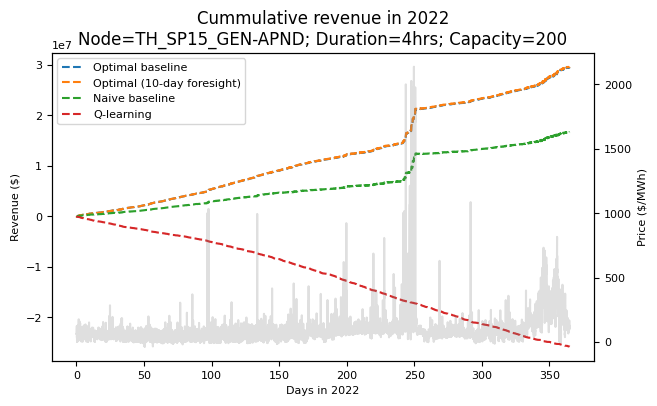
\includegraphics[width=.8\linewidth]{summ4hr.png}}
\end{figure}

\begin{figure}[htbp]
    \caption{\label{fig:summ100} 100-hr duration performance, by schedule}
\centerline{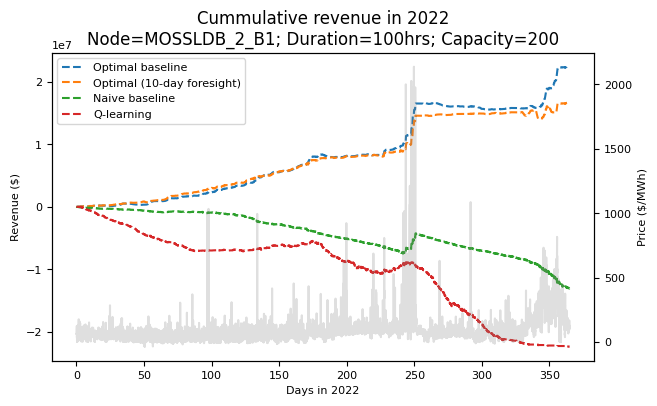
\includegraphics[width=.8\linewidth]{summ100hr.png}}
\end{figure}


\section{Discussion and conclusion}
From these results I make several conclusions. 
\begin{itemize}
    \item Long-duration batteries generate less revenue over a year than short-duration batteries, both in their theoretical optimal bounds and their naive baselines. While the short-duration batteries can still be profitable under a naive baseline, the long-duration batteries lose money.
    \item As expected, the optimal baselines under 10-day foresight are exactly the same as the optimal baselines under 1-year foresight for 4-hr duration batteries. This is not the case for long-duration batteries that can optimize behavior beyond a 10-day window.
    \item Without hyperparameter tuning, the reinforcement learning models underperform even the naive baselines, however with tuning I expect them to perform closer to the optimal bounds.
\end{itemize}

I identify several opportunities for the extension of this work
\begin{itemize}
    \item Improved price forecasting: The model-based reinforcement learning approach relies on price forecasts. In this project I use simple time-lagged OLS to make these forecasts, but they could be improved with other machine learnig models.
    \item Richer state space: I use available price data as well as indicators for time of day and year. Incorporating weather data, gas prices, and other correlated predictors could improve estimation of the value function.
    \item Improved efficiency and faster runtime: I worked with a large space of hyperparameters, leading to a large set of permutations to evaluate through cross validation. I expect that using higher-performing computing, and improving the efficiency of my algorithms can improve these results.
\end{itemize}
\section{Appendix tables and figures \label{sec:taf}}


% -------------------------------------------------
% <><><><><><><>    Timeseries
% -------------------------------------------------


\begin{figure}[h]
    \caption{\label{fig:ts} Timeseries model performance on validation year}
\centerline{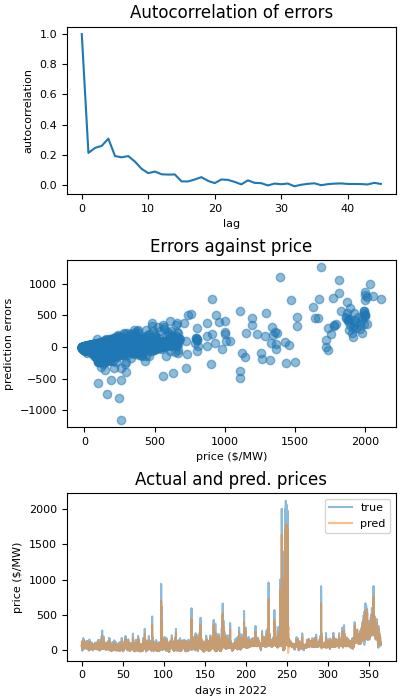
\includegraphics[width=0.8\linewidth]{timeseries.png}}
\end{figure}


\begin{table}[h]
    \caption{\label{tab:ts1} Regression results for $PRT_{t+1} \sim PRT_t + X$}
\begin{center}
    \begin{tabular}{lclc}
\hline
\textbf{Dep. Var:}           &        y         & \textbf{  R-sq:         } &       0.737    \\
\textbf{Model:}                   &       OLS        & \textbf{  Adj. R-sq:    } &       0.736    \\
\textbf{Method:}                  &  Least Squares   & \textbf{  F-stat:       } &       3914.    \\
\textbf{No. Obs:}        &       70073               & \textbf{  Prob (F-stat):} &       0.00     \\
\textbf{Df Res:}            &       70022      & \textbf{  Log-Li:    } &  -3.2620e+05   \\
\textbf{Df Model:}                &          50      & \textbf{  AIC:               } &   6.525e+05    \\
\textbf{Cov Type:}         &    nonrobust     & \textbf{  BIC:               } &   6.530e+05    \\
\hline
\end{tabular}
\end{center}
\end{table}

\begin{table}[htbp]
    \caption{\label{tab:ts2} Regression results for $PRT_{t+1} \sim PRT_t + X$, continued}
    \begin{center}
        \begin{tabular}{lccc}
            & \textbf{coef} & \textbf{std err} & \textbf{p-value} \\
\midrule
\textbf{lmp\_rt\_m1}              &       0.6862  &        0.009     & 0.000  \\
\textbf{lmp\_rt\_m1\_sq}          &     -4.6e-06  &     8.44e-06     & 0.586  \\
\textbf{lmp\_rt\_m2}              &       0.0223  &        0.009     & 0.019  \\
\textbf{lmp\_rt\_m2\_sq}          &   -2.805e-06  &     9.21e-06     & 0.761  \\
\textbf{lmp\_rt\_m3}              &       0.0573  &        0.009     & 0.000  \\
\textbf{lmp\_rt\_m3\_sq}          &    4.464e-06  &     9.23e-06     & 0.629  \\
\textbf{lmp\_rt\_m4}              &       0.2925  &        0.009     & 0.000  \\
\textbf{lmp\_rt\_m4\_sq}          &      -0.0002  &     9.14e-06     & 0.000  \\
\textbf{lmp\_rt\_m5}              &      -0.2004  &        0.009     & 0.000  \\
\textbf{lmp\_rt\_m5\_sq}          &    9.242e-05  &     9.24e-06     & 0.000  \\
\textbf{lmp\_rt\_m6}              &      -0.0353  &        0.009     & 0.000  \\
\textbf{lmp\_rt\_m6\_sq}          &    1.895e-05  &     9.21e-06     & 0.040  \\
\textbf{lmp\_rt\_m7}              &       0.0439  &        0.008     & 0.000  \\
\textbf{lmp\_rt\_m7\_sq}          &    3.593e-06  &     8.41e-06     & 0.669  \\
\textbf{lmp\_rt\_m84}             &       0.0275  &        0.004     & 0.000  \\
\textbf{lmp\_rt\_m85}             &      -0.0281  &        0.005     & 0.000  \\
\textbf{lmp\_rt\_m86}             &      -0.0188  &        0.005     & 0.000  \\
\textbf{lmp\_rt\_m87}             &      -0.0189  &        0.005     & 0.000  \\
\textbf{lmp\_rt\_m88}             &       0.0437  &        0.005     & 0.000  \\
\textbf{lmp\_rt\_m89}             &      -0.0175  &        0.005     & 0.000  \\
\textbf{lmp\_rt\_m90}             &      -0.0178  &        0.005     & 0.000  \\
\textbf{lmp\_rt\_m91}             &       0.0166  &        0.005     & 0.000  \\
\textbf{lmp\_rt\_m92}             &       0.1056  &        0.005     & 0.000  \\
\textbf{lmp\_rt\_m93}             &      -0.0918  &        0.005     & 0.000  \\
\textbf{lmp\_rt\_m94}             &       0.0236  &        0.005     & 0.000  \\
\textbf{lmp\_rt\_m95}             &       0.0784  &        0.004     & 0.000  \\
\textbf{lmp\_da}                  &       0.0465  &        0.004     & 0.000  \\
\textbf{node}                     &      -0.3573  &        0.209     & 0.088  \\
\textbf{h\_0}                     &      -0.2420  &        0.462     & 0.600  \\
\textbf{h\_1}                     &      -0.4694  &        0.461     & 0.309  \\
\textbf{h\_2}                     &      -0.2936  &        0.462     & 0.525  \\
\textbf{h\_3}                     &       0.0505  &        0.462     & 0.913  \\
\textbf{h\_4}                     &       0.7766  &        0.462     & 0.093  \\
\textbf{h\_5}                     &       1.2406  &        0.462     & 0.007  \\
\textbf{h\_6}                     &      -0.7611  &        0.464     & 0.101  \\
\textbf{h\_7}                     &      -2.3337  &        0.464     & 0.000  \\
\textbf{h\_8}                     &      -0.6525  &        0.467     & 0.162  \\
\textbf{h\_9}                     &      -0.3311  &        0.463     & 0.475  \\
\textbf{h\_10}                    &      -0.1346  &        0.463     & 0.771  \\
\textbf{h\_11}                    &       0.0772  &        0.463     & 0.868  \\
\textbf{h\_12}                    &       0.1238  &        0.463     & 0.789  \\
\textbf{h\_13}                    &       0.8018  &        0.464     & 0.084  \\
\textbf{h\_14}                    &       1.1200  &        0.467     & 0.016  \\
\textbf{h\_15}                    &       2.9921  &        0.472     & 0.000  \\
\textbf{h\_16}                    &       2.6390  &        0.474     & 0.000  \\
\textbf{h\_17}                    &       4.7740  &        0.476     & 0.000  \\
\textbf{h\_18}                    &       3.7959  &        0.479     & 0.000  \\
\textbf{h\_19}                    &      -6.1934  &        0.479     & 0.000  \\
\textbf{h\_20}                    &      -3.0551  &        0.478     & 0.000  \\
\textbf{h\_21}                    &      -1.8269  &        0.472     & 0.000  \\
\textbf{h\_22}                    &      -1.2875  &        0.467     & 0.006  \\
\textbf{h\_23}                    &      -1.1679  &        0.464     & 0.012  \\
\bottomrule
\end{tabular}
\end{center}
\end{table}

\bibliographystyle{IEEEtran}
\bibliography{IEEEabrv,egbib}

\vspace{12pt}

\end{document}
